\documentclass[
]{jss}

%% recommended packages
\usepackage{orcidlink,thumbpdf,lmodern}

\usepackage[utf8]{inputenc}

\author{
Łukasz Chrostowski\\Adam Mickiewicz University \And Piotr
Chlebicki~\orcidlink{0009-0006-4867-7434}\\Stockholm University
\AND Maciej Beręsewicz~\orcidlink{0000-0002-8281-4301}\\Poznań
University of Economics and Business\\
Statistical Office in Poznań
}
\title{\pkg{nonprobsvy} -- An R package for modern methods for
non-probability surveys}

\Plainauthor{Łukasz Chrostowski, Piotr Chlebicki, Maciej Beręsewicz}
\Plaintitle{nonprobsvy -- An R package for modern methods for
non-probability surveys}
\Shorttitle{\pkg{nonprobsvy} for non-probability surveys}


\Abstract{
The paper presents the \pkg{nonprobsvy} package which implements the
state-of-the-art statistical inference methods for non-probability
samples. The package implements various approaches that can be
categorized into three groups: prediction-based approach, inverse
probability weighting and doubly robust approach. On the contrary to the
existing packages \pkg{nonprobsvy} assumes existance of either full
population or probability-based population information and laverage the
\pkg{survey} package for the inference. The package implements both
analytical and bootstrap variance estimation for all of the proposed
estimators. In the paper we present the theory behind the package, its
functionalities and case study that showcases the usage of the package.
The package is aimed at official statisticans, public opinion or market
researchers who whould like to use non-probability samples (e.g.~big
data, opt-in web panels, social media) to accurately estimate popualtion
characteristics.
}

\Keywords{data integration, doubly robust estimation, propensity score
estimation, mass imputation, \pkg{survey}}
\Plainkeywords{data integration, doubly robust estimation, propensity
score estimation, mass imputation, survey}

%% publication information
%% \Volume{50}
%% \Issue{9}
%% \Month{June}
%% \Year{2012}
%% \Submitdate{}
%% \Acceptdate{2012-06-04}

\Address{
    Łukasz Chrostowski\\
    Adam Mickiewicz University\\
    First line\\
Second line\\
  E-mail: \email{lukchr@st.amu.edu.pl}\\
  URL: \url{https://posit.co}\\~\\
      Piotr Chlebicki\\
    Stockholm University\\
    Matematiska institutionen\\
Albano hus 1\\
106 91 Stockholm, Sweden\\
  E-mail: \email{piotr.chlebicki@math.su.se}\\
  URL: \url{https://github.com/Kertoo},
\url{https://www.su.se/profiles/pich3772}\\~\\
      Maciej Beręsewicz\\
    Poznań University of Economics and Business\\
Statistical Office in Poznań\\
    \hfill\break
Poznań University of Economics and Business\\
Department of Statistics\\
Institute of Informatics and Quantitative Economics\\
Al. Niepodległosci 10\\
61-875 Poznań, Poland\\
\strut \\
Centre for the Methodology of Population Studies\\
Statistical Office in Poznań\\
ul. Wojska Polskiego 27/29\\
60-624 Poznań, Poland\\
  E-mail: \email{maciej.beresewicz@ue.poznan.pl}\\
  URL: \url{https://github.com/BERENZ},
\url{https://ue.poznan.pl/en/people/dr-maciej-beresewicz/}\\~\\
  }


% tightlist command for lists without linebreak
\providecommand{\tightlist}{%
  \setlength{\itemsep}{0pt}\setlength{\parskip}{0pt}}




\usepackage{amsmath, amsthm, amssymb} \usepackage{calc, ragged2e} \usepackage[ruled]{algorithm2e} \usepackage{algpseudocode} \newcommand{\argmin}{\operatornamewithlimits{arg\,min}} \newcommand{\argmax}{\operatornamewithlimits{arg\,max}} \newcommand{\bX}{\boldsymbol{X}} \newcommand{\bx}{\boldsymbol{x}} \newcommand{\bY}{\boldsymbol{Y}} \newcommand{\by}{\boldsymbol{y}} \newcommand{\bh}{\boldsymbol{h}} \newcommand{\bH}{\boldsymbol{H}} \newcommand{\ba}{\boldsymbol{a}} \newcommand{\bp}{\boldsymbol{p}} \newcommand{\bA}{\boldsymbol{A}} \newcommand{\bw}{\boldsymbol{w}} \newcommand{\bd}{\boldsymbol{d}} \newcommand{\bZ}{\boldsymbol{Z}} \newcommand{\bz}{\boldsymbol{z}} \newcommand{\bv}{\boldsymbol{v}} \newcommand{\bu}{\boldsymbol{u}} \newcommand{\bU}{\boldsymbol{U}} \newcommand{\bQ}{\boldsymbol{Q}} \newcommand{\bG}{\boldsymbol{G}} \newcommand{\HT}{\text{\rm HT}} \newcommand{\bbeta}{\boldsymbol{\beta}} \newcommand{\balpha}{\boldsymbol{\alpha}} \newcommand{\btau}{\boldsymbol{\tau}} \newcommand{\bgamma}{\boldsymbol{\gamma}} \newcommand{\btheta}{\boldsymbol{\theta}} \newcommand{\blambda}{\boldsymbol{\lambda}} \newcommand{\bPhi}{\boldsymbol{\Phi}} \newcommand{\bEta}{\boldsymbol{\eta}} \newcommand{\bZero}{\boldsymbol{0}} \newcommand{\colvec}{\operatorname{colvec}} \newcommand{\logit}{\operatorname{logit}} \newcommand{\Exp}{\operatorname{Exp}} \newcommand{\Ber}{\operatorname{Bernoulli}} \newcommand{\Uni}{\operatorname{Uniform}}

\begin{document}



\section{Introduction}\label{sec-introduction}

In official statistics, information about the target population and its
characteristics is mainly collected through probability surveys, census
or is obtained from administrative registers, which covers all (or
nearly all) units of the population. However, owing to increasing
non-response rates, particularly unit non-response and non-contact,
resulting from the growing respondent burden, as well as rising costs of
surveys conducted by National Statistical Institutes, non-probability
data sources are becoming more popular
\citep{berkesewicz2017two, beaumont2020probability, biffignandi2021handbook}.
Non-probability surveys, such as opt-in web panels, social media,
scanner data, mobile phone data or voluntary register data, are
currently being explored for use in the production of official
statistics \citep{citro2014multiple, daas2015big}, public opinion
studies \citep{Schonlau2017} or market research \citep[cf.][]{Grow2022}.
Since the selection mechanism in these sources is unknown, standard
design-based inference methods cannot be directly applied and in case of
large datasets may lead to \textit{big data paradox} as described by
\citet{meng2018statistical}.

Table \ref{tab-comparison-characteristics} compares the basic
characteristics of probability and non-probability samples. In
particular, what are the advantages and disadvantages of each type with
respect to the selection mechanism, the population coverage, bias,
variance, costs and timeliness. In general, non-probability samples
suffers from unknown selection mechanism (i.e.~unknown probabilities of
inclusion) and under-coverage of certain groups from the population
(e.g.~older people). As a result, direct estimation based on
non-probability samples are characterised with bias and, in most cases,
small variance due to the sample size which leads to so called
\textit{big data paradox} i.e.~the larger the sample the larger the
bias. Certainly, cost and timeliness of these surveys is significantly
smaller than for non-probability samples.

\begin{table}[ht!]
    \centering
    \begin{tabular}{lll}
    \hline
    \textbf{Factor}   &  \textbf{Probability sample} & \textbf{Non-probability sample}\\
    \hline
    Selection & Known probabilities & Unknown self-selection \\
    Coverage & Complete & May be incomplete \\
    Estimation bias & Unbiased under design & Potential systematic bias \\
    Variance of estimates & Typically high & Typically low \\
    Cost & High & Low \\
    Timeliness & Long & Rapid \\
    \hline
    \end{tabular}
    \caption{Comparison of probability and non-probability samples and its characteristics}
    \label{tab-comparison-characteristics}
\end{table}

To address this problem, several approaches based on the estimation of
propensity scores (i.e.~inclusion probabilities) used to derive inverse
probability weights (IPW; also known as propensity score
weighting/adjustment, cf.~\citet{lee2006propensity, lee2009estimation}),
model-based prediction (in particular, mass imputation estimators; MI)
and doubly robust (DR) approach involving IPW and MI estimators has been
proposed for two main scenarios: 1) only population-level means or
totals are available, and 2) unit-level data is available either in the
form registers covering the whole population or in the form of
probability surveys \citep[cf.][]{elliott_inference_2017}.
\citet{wu2022statistical} classified these approaches into three groups
that require a joint randomization framework involving
\textit{probability sampling design} (denoted as \(p\)) and one of the
outcome regression model (denoted as \(\xi\)) or propensity score model
(denoted as \(q\)). In this approach the IPW estimators are under the
\(qp\) framework, the MI estimators are under the \(\xi p\) framework,
DR estimators are under the \(qp\) or \(\xi p\) framework.

Most approaches assume that population data are used to reduce the bias
of non-probability sampling by a proper reweighting to reproduce known
population totals/means (i.e.~IPW estimators); by modelling target
variable using various techniques (i.e.~MI estimators); or combining
both approaches (for instance DR estimators, cf.~\citet{chen2020doubly};
see also Multilevel Regression and Post-stratification, MRP;
\textit{Mister-P}, cf.~\citet{gelman1997poststratification}). This topic
have became very popular and number of new methods were proposed; for
instance non-parametric approaches based on nearest neighbours
\citep{yang2021integration}, kernel density estimation
\citep{chen_nonparametric_2022}, empirical likelihood
\citep{kim2023empirical}, model-calibration with LASSO \citep{chen2018}
or quantile balanced IPW \citep{beresewicz2025} to name a few. It should
be highlighted that, on contrary to probability samples, there is no
single method that can be used for non-probability samples. As shown
literature, and thus statistical software, offers various methods as
presented in the next section.

\subsection{Software for non-probability samples}\label{sec-software}

Table \ref{tab-comparisons} presents comparison of availability of
various inference methods for selected packages. We focused on packages
available through CRAN or PyPI (for non-CRAN or non-PyPI software see
\citet{cobo2024software}). In the comparison we have included four
packages that particularly focus on non-probability samples in
\proglang{R}: \pkg{NonProbEst} \citep{NonProbEst}, in \proglang{Python}
\pkg{balance} \citep{sarig2023balancepythonpackage}, \pkg{inps}
\citep{castro2024inps} and our \pkg{nonprobsvy}. In addition, we have
included two \proglang{R} packages that implements specific methods:
\pkg{rstanarm} (MRP; \citet{rstanarm}) and \pkg{GJRM} (generalized
sample selection models; \citet{GJRM}).

\begin{table}[ht!]
\centering
\resizebox{\linewidth}{!}{
\begin{tabular}{p{4cm}cccccc}
\hline
\textbf{Functionalities} & \pkg{NonProbEst} & \pkg{balance} & \pkg{inps} & \pkg{rstanarm} & \pkg{GJRM} & \pkg{nonprobsvy} \\
\hline
IPW  & $\checkmark$ & $\checkmark$ & $\checkmark$ & -- & ? & $\checkmark$ \\
Calibrated IPW  & -- & -- & -- & -- & -- & $\checkmark$ \\
MI & $\checkmark$ & -- & -- & -- & -- & $\checkmark$ \\
DR & -- & -- & $\checkmark$ & -- & -- & $\checkmark$\\
MRP & -- & -- & -- & $\checkmark$ & -- & -- \\
Sample selection & -- & -- & -- & -- & $\checkmark$ & -- \\
Variable selection & $\checkmark$ & $\checkmark$ & $\checkmark$ & $\checkmark$ & $\checkmark$ & $\checkmark$\\
Analytical variance & -- & -- & -- & -- & -- & $\checkmark$\\
Bootstrap variance & $\checkmark$ & -- & -- & -- & -- & $\checkmark$\\
Integration with \pkg{survey} or \pkg{samplics} & -- & -- & -- & -- & -- & $\checkmark$\\
\hline
\end{tabular}
}
\caption{Comparison of packages and implemented methods}
\label{tab-comparisons}
\end{table}

The \pkg{NonProbEst} is the most comprehensive package in comparison to
other discussed in this section. It allows for various techniques such
as IPW or prediction approaches (e.g.~model-calibrated). It allows for
several different setting of the IPW weights, variables selection and
the variance is estimated using leave-one-out Jackknife procedure.
Unfortunately the package is no longer developed (last update was in
2022) and some of the techniques are outdated or proved in the recent
literature to be inappropriate for non-probability samples. The package
also contains various functions aimed at specific methods and does not
allow to leverage the \pkg{survey} package for estimation. The
\pkg{balance} package focuses solely on the PS approach. It assumes that
the the population totals are known and the authors implemented variance
estimator of the weighted mean as a measure of uncertainty for the IPW
estimator. The weights for the IPW estimator are constructed using the
approach proposed by \citet{Schonlau2017}. The \pkg{inps} contains
supports unit-level data from probability sample or population,
implements IPW, MI and DR estimators, allows for variable selection and
is at very early stage of development. It also implements kernel
weighting and a simple bootstrap approach via the \pkg{scipy.stats}
module \citep{scipy2020}. Neither \pkg{balance} nor \pkg{ips} leverage
usage of the \pkg{samplics} module \citep{Diallo2021}. The \pkg{GJRM}
package is the only package that allows to estimate sample selection
models used widely for correction of selection bias in observational
studies (including not missing at random mechanism). Unfortunately, to
best of our knowledge there is no theory on how this approach can be
used for estimating population quantities nor to conduct statistical
inference. Finally, the MRP approach is implemented solely in the
\pkg{rstanarm} with variable selection specified by an appropriate
prior.

There are several advantages of the \pkg{nonprobsvy} package over the
discussed ones. First, the package implements state-of-the-art methods
recently proposed in the literature along with valid statistical
inference procedures. Second, the package implements other approaches
such as calibrated IPW (i.e.~PS weights match the population or
estimated totals), NN and PMM matching, various IPW and DR estimators
with possibility of selection of link functions for logistic regression.
Thirdly, the \pkg{nonprobsvy} leverage functionalities of the
\pkg{survey} package to account for the design of the probability
sample. Finally, we provide a user friendly API that mimics \code{glm}
or other functions known in \proglang{R} with one main function that
allows to specify the approach and estimators. To our knowledge the
\pkg{nonprobsvy} is the solely software (open or close) that allows for
such functionalities.

The remaining part of the paper is as follows. In Section
\ref{sec-methods} theory of the statistical inference based on
non-probability samples is presented. We provide basic set up and
introduce specific methods in separate subsections. In the paper we
\citet{wu2022statistical} notation. Section \ref{sec-package} the main
function and the package functionalities. Section
\ref{sec-data-analysis} presents a case study of integration of the
Polish Job Vacancy Survey with a voluntary admin data: Central Job
Offers Database with an aim on estimating number of companies with at
least vacancy offered on a single shift. Section \ref{sec-s3methods}
presents classes and \code{S3Methods} implemented in the package. Paper
finishes with summary and plans for the future works. In the Appendix,
Table \ref{tab-list-of-symbols} presents list of symbols and Section
\ref{sec-details} contains algorithms for selected MI estimators. In the
Replication Materials we include additional codes for specific
estimators described in the paper.

\section{Methods for non-probability samples}\label{sec-methods}

\subsection{Basic setup}\label{basic-setup}

Let \(U=\{1,..., N\}\) denote the target population consisting of \(N\)
labelled units. Each unit \(i\) has an associated vector of auxiliary
variables \(\boldsymbol{x}_{i}\) and the study (target) variable
\(y_{i}\). Let \(\{ (y_i, \boldsymbol{x}_i), i \in S_A\}\) be a dataset
of a non-probability sample \(S_A\) of size \(n_A\) and let
\(\left\{\left(\boldsymbol{x}_i, \pi_{i}^B\right), i \in S_B\right\}\)
be a dataset of a probability sample \(S_B\) of size \(n_B\), where only
information about variables \(\boldsymbol{x}\) and inclusion
probabilities \(\pi^B\) are known for all units in the population. Each
unit in the sample \(S_B\) has been assigned a design-based weight given
by \(d_i^B = 1/\pi_i^B\).

Let \(R_i^A=I(i \in S_A)\) and \(R_i^B=I(i \in S_B)\) be indicators of
inclusion into non-probability \(S_A\) and probability \(S_B\) sample
respectively and defined for all units in the target population. Let
\(\pi_i^A=P(R_i^A=1 \mid \boldsymbol{x}_i, y_i)=P(R_i^A=1 \mid \boldsymbol{x}_i)\)
be the propensity scores (PS) which characterize the sample \(S_A\)
inclusion and participation mechanisms. On the contrary to \(\pi_i^B\),
the \(\pi_i^A\) and \(d_i^A=1/\pi_i^A\) are unknown. This description of
the data is presented in a more concise form in Table
\ref{tab-two-sources}.

\begin{table}[ht!]
    \centering
    \resizebox{\linewidth}{!}{
    \begin{tabular}{llcccc} 
    \hline
    Sample & ID & Inclusion ($R$) & Design weight ($d$) & Covariates ($\boldsymbol{x}$) & Study variable ($y$) \\
    \hline
    Non-probability  & 1 & 1 & ? & $\checkmark$ & $\checkmark$ \\ 
    $S_A$ & $\vdots$ & $\vdots$ & $\vdots$ & $\vdots$ & $\vdots$ \\
    & $n_A$ & 1 & ? & $\checkmark$ & $\checkmark$ \\
    Probability  & 1 & 0 & $\checkmark$ & $\checkmark$ & ? \\
    $S_B$ & $\vdots$ & $\vdots$ & $\vdots$ & $\vdots$ & $\vdots$ \\ 
    & $n_B$ & 0 & $\checkmark$ & $\checkmark$ & ? \\                                     
    \hline     
    \end{tabular}
    }
    \caption{Two sample setting}
    \label{tab-two-sources}
\end{table}

The goal is to estimate a finite population mean
\(\mu_y=N^{-1}\sum_{i=1}^{N} y_{i}\) of the target variable \(y\). As
values of \(y_{i}\) are not observed in the probability sample, it
cannot be used to estimate the target quantity. Instead, one could try
combining the non-probability and probability samples to estimate
\(\mu_y\). Given the absence of a universally accepted methodology for
achieving this objective, the assumptions vary considerably, as outlined
by \citet{wu2022statistical}. However, the main assumptions that apply
to all presented in this section methods are:

\begin{itemize}
\item[A1] $R_i^A$ and the study variable $y_i$ are independent given the set of covariates $\boldsymbol{x}_i$ (i.e., $\left(R_i^A \perp y_i\right) \mid \boldsymbol{x}_i$; missing at random mechanism).
\item[A2] All the units in the target population have non-zero PS, i.e., $\pi_i^A>0$, $i=1,2, \ldots, N$ (i.e. no coverage error).
\item[A3] The indicator variables $R_1, R_2, \ldots, R_N$ are independent given the set of auxiliary variables $\left(\boldsymbol{x}_1, \boldsymbol{x}_2, \ldots, \boldsymbol{x}_N\right)$ (i.e. no clustering).
\end{itemize}

In addition, we assume no overlap between \(S_A\) and \(S_B\), and no
measurement error in \(y_i\) and \(\boldsymbol{x}_i\) is observed.
Setting presented in Table \ref{tab-two-sources} may be also extended to
calibrated \(d_i^B\) weights (i.e.~\(d_i^B\) adjusted for
under-coverage, non-contact or non-response;
cf.~\cite{sarndal2005estimation}) but this requires additional
developments in the theory about the consistency of the MI, IPW and DR
estimators. In the next sections we briefly present methods that are
implemented in the package.

\subsection{Prediction-based approach}\label{sec-prediction}

\subsubsection{Prediction estimators}\label{prediction-estimators}

In the prediction approach the following semiparametric model for the
finite population is assumed

\begin{equation}
E_{\xi}\left(y_i \mid \boldsymbol{x}_i\right)=m\left(\boldsymbol{x}_i, \boldsymbol{\beta}\right), \text { and } \quad V_{\xi}\left(y_i \mid \boldsymbol{x}_i\right)=v\left(\boldsymbol{x}_i\right) \sigma^2, \quad i=1,2, \ldots, N,
\label{eq-semipar-model}
\end{equation}

where the mean function \(m(\cdot,\cdot)\) and the variance \(v(\cdot)\)
have known forms and it assumed that \(y_i\) are independent given
\(\boldsymbol{x}_i\). The model \eqref{eq-semipar-model} is assumed to
hold for all units in the non-probability sample \(S_A\). Parameters of
the \eqref{eq-semipar-model} can be estimated using quasi maximum
likelihood estimation method which covers linear and non-linear models
such as generalized linear models (GLM). Let \(\boldsymbol{\beta}_0\)
and \(\sigma^2_0\) be the true values of the model parameters
\(\boldsymbol{\beta}\) and \(\sigma^2\) under assumed model and the
\(\hat{\boldsymbol{\beta}}\) be the quasi maximum likelihood estimator
of \(\boldsymbol{\beta}_0\). Let
\(m_i=m(\boldsymbol{x}_i, \boldsymbol{\beta}_0)\) and
\(\hat{m}_i=m(\boldsymbol{x}_i, \hat{\boldsymbol{\beta}})\) for all
units \(i=1,...,N\). Under this settings, \citet{wu2022statistical}
notes there are two commonly used prediction estimators

\begin{equation}
\hat{\mu}_{y,PR1}=\frac{1}{N} \sum_{i=1}^N \hat{m}_i \quad \text { and } \quad \hat{\mu}_{y,PR2}=\frac{1}{N}\left\{\sum_{i \in S_A} y_i-\sum_{i \in S_A} \hat{m}_i+\sum_{i=1}^N \hat{m}_i\right\}.
\label{eq-pred-two-estimators}
\end{equation}

Under linear models where
\(m(\boldsymbol{x}_i, \boldsymbol{\beta})=\boldsymbol{x}_i^{\prime}\boldsymbol{\beta}\),
the two estimators \eqref{eq-pred-two-estimators} reduce to

\begin{equation}
\hat{\mu}_{y,PR1}=\mu_{\boldsymbol{x}}^{\prime} \hat{\boldsymbol{\beta}} \quad \text { and } \quad \hat{\mu}_{y,PR2}=\frac{n_A}{N}\left(\bar{y}_A-\overline{\boldsymbol{x}}_A^{\prime} \hat{\boldsymbol{\beta}}\right)+\mu_{\boldsymbol{x}}^{\prime} \hat{\boldsymbol{\beta}},
\label{eq-pred-two-estimators-simplified}
\end{equation}

where \(\mu_{\boldsymbol{x}} = N^{-1}\sum_{i=1}^N\boldsymbol{x}_i\) is
the vector of the population means of the \(\boldsymbol{x}\) variables
and
\(\overline{\boldsymbol{x}}_A=n_A^{-1}\sum_{i \in S_A}\boldsymbol{x}_i\)
is the vector of the simple means of \(\boldsymbol{x}\) from the
non-probability sample \(S_A\). If the linear model contains an
intercept and \(\hat{\boldsymbol{\beta}}\) is the ordinary least square
estimator then \(\hat{\mu}_{y,PR1}=\hat{\mu}_{y,PR2}\).

This form is appealing as the only requirement is the availability of a
non-probability sample \(S_A\) and reference population means (or totals
and population size \(N\)). If the population means are unknown they can
be replaced by estimates provided by the reference probability sample
\(S_B\) i.e.~\(\sum_{i=1}^N \hat{m}_i\) is replaced with
\(\sum_{i \in S_B} d_i^B\hat{m}_i\) for \eqref{eq-pred-two-estimators}
and \(\mu_{\boldsymbol{x}}\) is replaced by
\(\hat{\mu}_{\boldsymbol{x}}=\hat{N}_B^{-1}\sum_{i \in S_B}d_i^B\boldsymbol{x}_i\)
for \eqref{eq-pred-two-estimators-simplified} where
\(\hat{N}_B=\sum_{i \in S_B}d_i^B\).

\subsubsection{Mass imputation
estimators}\label{mass-imputation-estimators}

Model-based prediction estimators of \(\mu\) can be treated as
\textit{mass imputation estimators} as the information on \(y_i\) is
missing entirely in the reference probability sample \(S_B\) (but
\(\boldsymbol{x}_i\) is available) and \(y_i\) can be imputed based on
the non-probability sample as
\(\{ (y_i, \boldsymbol{x}_i), i \in S_A\}\) is observed. The general for
of the MI estimator is given by

\begin{equation}
\hat{\mu}_{y,MI}=\frac{1}{\hat{N}_{B}} \sum_{i \in S_{B}} d_i^{B} y_i^*, 
\end{equation}

where \(y_i^*\) is the imputed value of \(y_i\) and \(\hat{N}_{B}\) is
defined as previously. Under deterministic regression imputation the
\(\hat{\mu}_{y,MI}\) estimator reduce to \eqref{eq-pred-two-estimators}
estimators.

There are several approaches how to impute \(y_i^*\) and in the package
we have implemented the following MI estimators: semiparametric approach
based on the generalized linear models (MI-GLM), nearest neighbour
matching (MI-NN) and predictive mean matching (MI-PMM).

The properties of the MI-GLM estimator where \(y_i^*\) are \(\hat{m}_i\)
from the semiparametric model was studied by \citet{kim_combining_2021}.
In the \pkg{nonprobsvy} package we allow for the following GLM families:
\code{gaussian}, \code{binomial} and \code{poisson}.

The MI-NN estimator was initially proposed by \citet{rivers2007sampling}
under the name \textit{sample matching} and theoretical properties for
the MI-NN estimator for large non-probability samples (big data,
i.e.~covering a significant part of the target population) was studied
by \citet{yang2021integration}. The basic idea of the NN matching is as
follows: 1) for each \(i\) unit in the probability sample \(S_B\) find a
donor \(j\) (or donors) in sample \(S_A\) based on some distance between
\(\boldsymbol{x}_i\) and \(\boldsymbol{x}_j\); 2) use the matched values
\(y_j\) from \(S_A\) to impute missing \(y_i\) values in the probability
sample \(S_B\). Imputed values \(y_i^*\) depends on the number of
selected \(k\) neighbours, for \(k=1\) the closest one is selected and
for \(k>1\) a simple average over a vector of selected \(y\) may be
calculated. The detailed description is presented in the Algorithm
\ref{algo-2} in the Appendix. The MI-NN estimator suffers from the curse
of dimensionality as proved by for i.e.~asymptotic bias of the MI
estimator increases as the number of covariates \(\boldsymbol{x}\)
increases with a fixed \(k\)
\citep{abadie2006large, yang_asymptotic_2020}. To overcome this issue
PMM approach was proposed.

In the PMM approach matching is done using the predicted values of
\(\hat{m}_i=m\left(\boldsymbol{x}_i, \hat{\boldsymbol{\beta}}\right)\)
instead of \(\boldsymbol{x}_i\), thus the NN algorithm is modified as
follows: 1) fit the
\(m\left(\boldsymbol{x}_i, \boldsymbol{\beta}\right)\) to
non-probability sample \(S_A\), 2) assign predicted values \(\hat{m}_i\)
to all units in \(S_A\) and \(S_B\); 3) match all units from sample
\(S_B\) to donor units from sample \(S_A\) based on \(\hat{m}\) values.
The MI-PMM estimator is the same as in the NN approach.
\citet{chlebicki2025} studied properties of two variants of the MI-PMM
estimator for non-probability samples: matching predicted to predicted
(\(\hat{m}-\hat{m}\) matching; denoted as MI-PMM A) and predicted to
observed (\(\hat{m}-y\) matching; denoted as MI-PMM B). Details about
the procedure can be found in Algorithm \ref{algo-3} and \ref{algo-4} in
the Appendix. \citet{chlebicki2025} also prove consistency of the MI-PMM
A estimator under model mis-specification i.e.~the assumed model may be
different from the true one.

\subsubsection{Variance estimators for the prediction
approach}\label{variance-estimators-for-the-prediction-approach}

Variance for the MI estimators can be either estimated using analytical
or bootstrap approach. Analytical estimator of the variance of the
MI-GLM estimator proposed by \citet[p. 950]{kim_combining_2021} which
contains two components: \(\hat{V}_1\) (based on the information from
both samples \(S_A\) and \(S_B\)) and \(\hat{V}_2\) (based solely on the
probability sample \(S_B\)); for the MI-NN estimator
\citet{yang2021integration} proposed variance estimator for large
\(S_A\) samples which reduces to the probability sample \(S_B\) part
(i.e.~design-based variance estimator of the mean which can be easily
obtained from the \pkg{survey} package) and a proposal for smaller
samples can be found in \citet{chlebicki2025}; and for the MI-PMM
estimators \citet{chlebicki2025} contains formulas for variance
estimators which are the same as for the MI-PMM estimators.

The second approach is based on the bootstrap where in each bootstrap
replication \(b=1,...,B\) the following steps are conducted.

\begin{enumerate}
\item Independently:
  \begin{itemize}
  \item draw a simple random sampling with replacement from the non-probability sample $S_A$,
  \item draw a sample according to the declared sampling design from the probability sample $S_B$ (e.g. one can use \code{as.svrepdesign} function from the \pkg{survey} package).
  \end{itemize}
\item Estimate $\mu_{y, MI}^b$ based on appropriate approach (e.g. MI-GLM, MI-NN or MI-PMM).
\end{enumerate}

After obtaining \(B\) bootstrap replicates estimate variance based on
the following equation

\begin{equation}
\hat{V}_{\text{boot}} = \frac{1}{B-1}\sum_{b=1}^B\left(\hat{\mu}^b_y - \hat{\mu}_y\right)^2,
\label{eq-var-bootstrap}
\end{equation}

where \(\hat{\mu}_y\) is the estimated mean using either MI-GLM, MI-NN
or MI-PMM estimator.

The above approaches are applied when unit-level data from the
probability sample \(S_B\) are available. If this is not the case and
only population means (or totals and population size) we can estimate
variance of the \(\mu_{y,MI-GLM}\) estimator using the first component
\(\hat{V}_1\) of the \citet{kim_combining_2021} variance estimator
(replaced by the survey based population quantities if available). For
the variance of the MI-NN and MI-PMM estimators we only allow the
bootstrap approach with known population means. Note, that current
version of the \pkg{nonprobsvy} does not support the replicated weights
in the probability sample \(S_B\) for any of the estimators discussed in
this paper.

\subsection{Inverse Probability Weighting}\label{sec-ipw}

Another popular approach is inverse probability weighting (IPW) that
involves estimation of PS given by \(\pi_i^A=P\left(i \in S_A \right)\).
Similarly as for the prediction approach we have two variants of the IPW
estimator given by

\begin{equation}
\hat{\mu}_{y,IPW1}=\frac{1}{N} \sum_{i \in S_A} \frac{y_i}{\hat{\pi}_i^A} \quad \text { and } \quad \hat{\mu}_{y,IPW2}=\frac{1}{\hat{N}^A} \sum_{i \in S_A} \frac{y_i}{\hat{\pi}_i^A},
\label{eq-ipw-estimators}
\end{equation}

where the \(\hat{\mu}_{y,IPW1}\) is a version of the Horvitz-Thompson
estimator and the \(\hat{\mu}_{y,IPW2}\) is the Hájek estimator with the
estimated population size given by
\(\hat{N}^A = \sum_{i \in S_A} (\pi_i^A)^{-1}\). This estimator in the
case of non-probability samples was discussed by
\citet{lee2006propensity} and
\citet[chapter 13]{biffignandi2021handbook} and several approaches on
using propensity scores and alternative versions of the weights were
discussed \citep[cf.][section 3]{elliott_inference_2017} Recently,
\citet{chen2020doubly} studied properties of the
\eqref{eq-ipw-estimators} estimators, proved their consistency as well
as derived closed form estimators.
\citet[section 4.2]{wu2022statistical} argue that \(\hat{\mu}_{y,IPW2}\)
estimator performs better than \(\hat{\mu}_{y,IPW1}\) even if the
population size is known.

The construction of the IPW estimator involved two steps: 1) estimation
of the PS; and 2) deriving \(d_i^A\), which in our case are equal to
\(1/\pi_i^A\). To estimate the propensity scores
\(\pi_i^A=\pi(\boldsymbol{x}_i, \boldsymbol{\gamma})\) one can use the
likelihood approach under assumption that the information about
\(\boldsymbol{x}_i\) are available for each unit in the population given
by \eqref{eq-ipw-loglik}.

\begin{equation}
\ell(\boldsymbol{\gamma}) = \log\left\{\prod_{i=1}^N \left(\pi_i^A\right)^{R_i}\left(1-\pi_i^A\right)^{1-R_i}\right\} =
\sum_{i \in S_{A}} \log \left\{\frac{\pi\left(\boldsymbol{x}_i, \boldsymbol{\gamma}\right)}{1-\pi\left(\boldsymbol{x}_i, \boldsymbol{\gamma}\right)}\right\}+\sum_{i=1}^N \log \left\{1-\pi\left(\boldsymbol{x}_i, \boldsymbol{\gamma}\right)\right\}.
\label{eq-ipw-loglik}
\end{equation}

In practice, a function of this form cannot be used because we do not
observe all units from the population. More realistic approach involves
a reference probability sample \(S_B\) and as a result the second
component of the \eqref{eq-ipw-loglik} is replaced forming pseudo
log-likelihood function given by \eqref{eq-ipw-pseudo-loglik}

\begin{equation}
\ell^*(\boldsymbol{\gamma}) = \sum_{i \in S_{A}} \log \left\{\frac{\pi\left(\boldsymbol{x}_i, \boldsymbol{\gamma}\right)}{1-\pi\left(\boldsymbol{x}_i, \boldsymbol{\gamma}\right)}\right\}+ \sum_{i \in S_{B}} d_i^B \log \left\{1-\pi\left(\boldsymbol{x}_i, \boldsymbol{\gamma}\right)\right\}.
\label{eq-ipw-pseudo-loglik}
\end{equation}

The maximum pseudo-likelihood estimator \(\hat{\boldsymbol{\gamma}}\)
can be obtained as the solution to the pseudo score equation which under
logit function assumed for \(\pi_i^A\) is given by
\eqref{eq-ipw-solution-mle}

\begin{equation}
\boldsymbol{U}(\boldsymbol{\gamma}) = \sum_{i \in S_A} \boldsymbol{x}_i - \sum_{i \in S_B} d_i^B \pi(\boldsymbol{x}_i, \boldsymbol{\gamma}) \boldsymbol{x}_i.
\label{eq-ipw-solution-mle}
\end{equation}

In general, the pseudo score functions
\(\boldsymbol{U}(\boldsymbol{\gamma})\) at the true values of the model
parameters \(\boldsymbol{\gamma}_0\) are unbiased under the joint
\(q p\) randomization in the sense that
\(E_{q p}\left\{\boldsymbol{U}\left(\boldsymbol{\gamma}_0\right)\right\}=\boldsymbol{0}\),
which implies that the estimator \(\hat{\boldsymbol{\alpha}}\) is
\(qp\)-consistent for \(\boldsymbol{\gamma}_0\)
\citep{wu2022statistical}.

The system \eqref{eq-ipw-solution-mle} can be replaced by a system of
general estimation equations. Let
\(\boldsymbol{h}(\boldsymbol{x}, \boldsymbol{\gamma})\) be a
user-specified vector of functions with the same dimension of
\(\boldsymbol{\gamma}\) and \(\boldsymbol{G}(\boldsymbol{\gamma})\) is
defined as

\begin{equation}
\label{gee}
\boldsymbol{G}(\boldsymbol{\gamma})=\sum_{i \in S_A} \boldsymbol{h}\left(\boldsymbol{x}_i, \boldsymbol{\gamma}\right)-\sum_{i \in S_B} d_i^B \pi\left(\boldsymbol{x}_i, \boldsymbol{\gamma}\right) \boldsymbol{h}\left(\boldsymbol{x}_i, \boldsymbol{\gamma}\right),
\end{equation}

then solving \(\boldsymbol{G}(\boldsymbol{\gamma})=\boldsymbol{0}\) with
the chosen parametric form of \(\pi_i^A\) and the chosen
\(\boldsymbol{h}(\boldsymbol{x},\boldsymbol{\gamma})\) leads to the
consistent estimator of \(\hat{\boldsymbol{\gamma}}\). In the
literature, the most commonly considered functions are
\(\boldsymbol{h}\left(\boldsymbol{x}_i, \boldsymbol{\gamma}\right) = \boldsymbol{x}_i\)
and
\(\boldsymbol{h}\left(\boldsymbol{x}_i, \boldsymbol{\gamma}\right) = \boldsymbol{x}_i \pi\left(\boldsymbol{x}_i, \boldsymbol{\gamma}\right)^{-1}\).
Note that if the function \(\boldsymbol{h}_i=\boldsymbol{x}_i\), then
\(\boldsymbol{G}\) is reduced to

\[
\boldsymbol{G}(\boldsymbol{\gamma}) = \sum_{i \in S_A} \boldsymbol{x}_i-\sum_{i \in S_B} d_i^B \pi\left(\boldsymbol{x}_i, \boldsymbol{\gamma}\right) \boldsymbol{x}_i,
\]

and for the second variant of the \(\boldsymbol{h}\) function we get the
following form of the function \(\boldsymbol{G}\)

\begin{equation}
\boldsymbol{G}(\boldsymbol{\theta}) = \sum_{i \in S_A} \frac{\boldsymbol{x}_i}{\pi\left(\boldsymbol{x}_i, \boldsymbol{\gamma}\right) }-\sum_{i \in S_B} d_i^B \boldsymbol{x}_i,
\label{eq-ipw-solution-gee}
\end{equation}

which can be viewed as \textit{calibrated} IPW and equation
\eqref{eq-ipw-solution-gee} requires only the knowledge of population
totals for the auxiliary variables \(\boldsymbol{x}\). Moreover, usage
of the \eqref{eq-ipw-solution-gee} leads to doubly robust estimator
under assumption that the outcome model is linear
\citep{kim_theory_2012}.

\subsubsection{Variance estimators for the inverse probability weighting
approach}\label{variance-estimators-for-the-inverse-probability-weighting-approach}

\citet[section 3.2]{chen2020doubly} derived asymptotic variance
estimators for both IPW estimators presented in
\eqref{eq-ipw-estimators} and presented the plug-in variance estimator
for the \(\hat{\mu}_{y,IPW2}\) estimator assuming logistic regression.
In the package we have implemented this approach for \code{logit},
\code{probit} and \code{cloglog} link functions. We refer the reader to
the \citet[section 6.2]{wu2022statistical} and
\citet[chapter 3]{chrostowski2024statistical} for more details on how
this estimators are derived based on the general estimating equations
approach.

Another approach is to use bootstrap which essentially is the same as
the one presented in the \eqref{eq-var-bootstrap} where the
\(\hat{\mu}_y\) is replaced by one of the \eqref{eq-ipw-estimators}
estimators.

\subsection{Doubly Robust approach}\label{sec-dr-approach}

The IPW and MI estimators are sensible to mis-specified models for PS
and outcome respectively. To improve robustness and efficiency, the DR
approach was proposed \citep[cf.][]{robins1994estimation}. It
incorporates a prediction model for the response variable \(y_i\) and PS
model for participation \(R_i^A\). This approach is doubly robust in
that sense that the DR estimator remains consistent even if one of the
models is mis-specified. We need to consider a joint randomization
approach consisting of a non-probability \(S_A\) and probability \(S_B\)
sample and DR inference is done within the \(qp\) or \(\xi p\) framework
with no specification which one is correct. The general formulae for the
for the DR estimator is given by

\[
\tilde{\mu}_{y,DR} = \frac{1}{N}\sum_{i \in S_A}\frac{y_i - m_i}{\pi_i^A} + \frac{1}{N}\sum_{i =1}^N m_i,
\]

where \(\pi_i^A\) and \(m_i\) are defined as previously. In the next
subsections we discuss two approaches to the DR estimation.

\subsubsection{Parameters estimated
separately}\label{parameters-estimated-separately}

\citet{chen2020doubly} proposed two DR estimators given in
\eqref{eq-dr-known-n} and \eqref{eq-dr-estimated-n} under assumption
that population size either known or estimated

\begin{equation}
\hat{\mu}_{y,DR1}=\frac{1}{N} \sum_{i \in S_{A}} d_i^{A}\left\{y_i-m\left(\boldsymbol{x}_i, \hat{\boldsymbol{\beta}}\right)\right\}+\frac{1}{N} \sum_{i \in S_{B}} d_i^{B} m\left(\boldsymbol{x}_i, \hat{\boldsymbol{\beta}}\right),
\label{eq-dr-known-n}
\end{equation}

and

\begin{equation}
\hat{\mu}_{y,DR2}=\frac{1}{\hat{N}^{A}} \sum_{i \in S_{A}} d_i^{A}\left\{y_i-m\left(\boldsymbol{x}_i, \hat{\boldsymbol{\beta}}\right)\right\}+\frac{1}{\hat{N}^{B}} \sum_{i \in S_{B}} d_i^{B} m\left(\boldsymbol{x}_i, \hat{\boldsymbol{\beta}}\right),
\label{eq-dr-estimated-n}
\end{equation}

where
\(d_i^A=\pi\left(\boldsymbol{x}_i, \boldsymbol{\gamma}\right)^{-1}, \hat{N}^A=\sum_{i \in S_A} d_i^A\)
and \(\hat{N}^B=\sum_{i \in S_B} d_i^B\). The estimator
\eqref{eq-dr-estimated-n} using the estimated population size has better
performance in terms of bias and mean squared error and should be used
in practice. However, the main limitation is estimation of the variance
which will be discussed at the end of this section.

\citet{chen2020doubly} suggested to construct the \eqref{eq-dr-known-n}
or \eqref{eq-dr-estimated-n} estimator based on the two models estimated
separately which is attractive as it is possible to specify different
number of variables for the propensity and outcome model. An alternative
approach was proposed by \citet{yang_doubly_2020}, similar to
\citet{kim2014doubly} and will be discussed in the next subsection.

\subsubsection{Minimization of the bias for doubly robust
methods}\label{minimization-of-the-bias-for-doubly-robust-methods}

\citet{yang_doubly_2020} discussed variable selection for
high-dimensional setting and noted that we cannot control the bias of
the estimator, which may increase. Therefore, according to
\citet{yang_doubly_2020}, the idea is to determine the equations leading
to the estimation of the \(\boldsymbol{\beta}\) and
\(\boldsymbol{\gamma}\) parameters based on the bias of the population
mean estimator. This method allows for the estimation of the parameters
\(\boldsymbol{\beta}\) and \(\boldsymbol{\gamma}\) in a single step,
rather than in two separate steps. First, they derived the bias of the
\(\hat{\mu}_{DR}\), assuming
\(\boldsymbol{h}(\boldsymbol{x}, \boldsymbol{\gamma})=\boldsymbol{x}\pi(\boldsymbol{x}, \boldsymbol{\gamma})^{-1}\)
for the IPW estimator, which is given by equation \eqref{eq-dr-bias}

\begin{equation}
\begin{aligned}
\operatorname{bias}\left(\hat{\mu}_{D R}\right) = \mid\hat{\mu}_{DR}-\mu\mid &=\frac{1}{N} \sum_{i=1}^N\left\{\frac{R_i^A}{\pi\left(\boldsymbol{x}_i, \boldsymbol{\gamma}\right)} - 1\right\}\left\{y_i-m\left(\boldsymbol{x}_i, \boldsymbol{\beta}\right)\right\}\\
& + \frac{1}{N} \sum_{i=1}^N\left(R_i^B d_i^B-1\right) m\left(\boldsymbol{x}_i, \boldsymbol{\beta}\right)
\end{aligned}
\label{eq-dr-bias}
\end{equation}

The goal of this approach is to minimize
\(\operatorname{bias}\left(\hat{\mu}_{D R}\right)^2\) which leads to
solving the following system of equations

\begin{equation}
\left(\begin{array}{c}
\sum_{i=1}^N R_i^A\left\{\frac{1}{\pi\left(\boldsymbol{x}_i, \boldsymbol{\gamma}\right)}-1\right\}\left\{y_i-m\left(\boldsymbol{x}_i, \boldsymbol{\beta}\right)\right\} \boldsymbol{x}_i \\
\sum_{i=1}^N \frac{R_i^A}{\pi\left(\boldsymbol{x}_i, \boldsymbol{\gamma}\right)} \dot{m}\left(\boldsymbol{x}_i, \boldsymbol{\beta}\right) -\sum_{i \in S_{\mathrm{B}}} d_i^{\mathrm{B}} \dot{m}\left(\boldsymbol{x}_i, \boldsymbol{\beta}\right)
\end{array}\right) = \boldsymbol{0},
\label{eq-bias-min}
\end{equation}

where
\(\dot{m}\left(\boldsymbol{x}_i, \boldsymbol{\beta}\right)=\frac{\partial m\left(\boldsymbol{x}_i, \boldsymbol{\beta}\right)}{\partial \boldsymbol{\beta}}\)
and system \eqref{eq-bias-min} can be solved using Newton--Raphson
method. This approach, without variable selection, is equivalent to
\citet{kim2014doubly} and was extensively discussed by
\citet{chen2020doubly} and \citet{wu2022statistical} in the context of
estimation of parameters and its variance estimator. The main limitation
is the existence of the solution to \eqref{eq-bias-min} as it may not
exist unless the two sets of covariates used, respectively, in the
outcome regression model and the PS model have the same dimensions. That
is why \citet{yang_doubly_2020} suggested to use this approach on a
union of variables from both models (e.g.~after variable selection).

In the \pkg{nonprobsvy} package we have implemented these approaches not
only for
\(\boldsymbol{h}(\boldsymbol{x}, \boldsymbol{\gamma})=\boldsymbol{x}_i \pi\left(\boldsymbol{x}_i, \boldsymbol{\gamma}\right)^{-1}\)
but also for
\(\boldsymbol{h}(\boldsymbol{x}, \boldsymbol{\gamma})=\boldsymbol{x}\)
and various link functions for propensity score model. We also allow
selection of this estimation strategy with or without variable selection
methods discussed in Section \ref{sec-varsel}. As noted in the beginning
the selection between \eqref{eq-dr-known-n} and
\eqref{eq-dr-estimated-n} result in a different approach of estimating
variance which will be presented in the next subsection.

\subsubsection{Variance estimators for the doubly robust
approach}\label{variance-estimators-for-the-doubly-robust-approach}

\citet{yang_doubly_2020} derived a closed form estimator for the
\eqref{eq-dr-known-n} but this requires knowledge of the population and
it is requires bias correction to obtain valid estimator for
\(V_{\xi p}\left(\hat{\mu}_{y,DR}-\mu_y\right)\) under the outcome
regression model \(\xi\). A doubly robust variance estimator for the
\(\hat{\mu}_{y,DR2}\) given by \eqref{eq-dr-estimated-n} is not yet
available in the literature. In the package, for the analytical variance
estimator of the \(\hat{\mu}_{y,DR2}\) we simply replace \(N\) with
estimated \(\hat{N}_A\) and \(\hat{N}_B\) and we strongly advice users
to be be careful when using this approach.

Alternatively, one can use the bootstrap approach.
\citet{chen2020doubly} showed that bootstrap approach presented in the
Section \ref{sec-prediction} have good performance in terms of coverage
rate when one of the working models is correctly specified. That is why
this approach is recommended for all users.

\subsection{Variable selection algorithms}\label{sec-varsel}

\citet{yang_asymptotic_2020} point that using variable selection
techniques during estimation is crucial, especially when dealing with
high-dimensional non-probability sample. Variable selection not only
improves the model stability and computational feasibility, but also
reduces the variance, which can increase when irrelevant auxiliary
variables are included.

The most popular approaches in the statistical literature are
penalisation methods such as
\textit{Least Absolute Shrinkage and Selection Operator} (LASSO),
\textit{Smoothly Clipped Absolute Deviation} (SCAD) or
\textit{Minimax Concave Penalty} (MCP), which, thanks to appropriate
loss functions, degenerate the coefficients in variables that have no
significant effect on the dependent variable
\citep[cf.][]{tibshirani1996regression, ncvreg}.

The selection procedure works in a similar way for non-probability
methods with loss functions modified to take into account external data
sources such as sample or population totals or averages. In particular,
the technique is divided into two steps: 1) we select the relevant
variables using an appropriately constructed loss function (and possibly
using the \eqref{eq-bias-min} approach to obtain the final estimates of
the model parameters); and 2) we construct chosen estimator using
variables selected from the first step. For instance,
\citet{yang_doubly_2020} used \eqref{eq-varsel-loss-mi} as a loss
function for estimating outcome equation parameters

\begin{equation}  
\operatorname{Loss}\left(\lambda_{\boldsymbol{\beta}}\right)=\sum_{i=1}^N R_i^A\left[y_i-m\left\{\boldsymbol{x}_i, \boldsymbol{\beta}(\lambda_{\boldsymbol{\beta}})\right\}\right]^2,
\label{eq-varsel-loss-mi}
\end{equation}

where
\(m\left\{\boldsymbol{x}_i, \boldsymbol{\beta}(\lambda_{\boldsymbol{\beta}})\right\}\)
is the penalized function for the \(\boldsymbol{\beta}\) parameters with
a tuning parameter \(\lambda_{\boldsymbol{\beta}}\) and loss functions
for the PS function presented in the Table \ref{tab-varsel-loss-ipw}
where \(\lambda_{\boldsymbol{\gamma}}\) is the tuning parameter.

\begin{table}[ht!]
\centering
\begin{tabular}{ll}
\hline
$\boldsymbol{h}(\boldsymbol{x}_i, \boldsymbol{\gamma})$ function &  Loss function $\lambda_{\boldsymbol{\gamma}}$ \\
\hline
$\boldsymbol{x}_i$ & $\sum_{j=1}^p\left(\sum_{i=1}^N\left[R_i^A - \frac{R^B\pi\left\{\boldsymbol{x}_i, \boldsymbol{\gamma}(\lambda_{\boldsymbol{\gamma}})\right\}}{\pi_i^B}\right] \boldsymbol{x}_{i, j}\right)^2$\\
\hline
$\boldsymbol{x}_i \pi_i(\boldsymbol{x}_i, \boldsymbol{\gamma})^{-1}$ & $\sum_{j=1}^p\left(\sum_{i=1}^N\left[\frac{R_i^A}{\pi\left\{\boldsymbol{x}_i, \boldsymbol{\gamma}(\lambda_{\boldsymbol{\gamma}})\right\}}-\frac{R_i^B}{\pi_i^B}\right] \boldsymbol{x}_{i, j}\right)^2$ \\
\hline
\end{tabular}
\caption{Loss functions for the PS function depending on the $\boldsymbol{h}(\cdot,\cdot)$ function}
\label{tab-varsel-loss-ipw}
\end{table}

where \(R_i^A\) and \(R_i^B\) are indicator functions defining the
inclusion into non-probability \(S_A\) and probability \(S_B\) samples
respectively. \citet{yang_doubly_2020} discussed only the SCAD penalty
and the
\(\boldsymbol{h}(\boldsymbol{x}_i, \boldsymbol{\gamma})=\boldsymbol{x}_i\)
function for the DR estimator only. In the \pkg{nonprobsvy} package we
have extended this approach to first variant of the
\(\boldsymbol{h}(\boldsymbol{x}_i, \boldsymbol{\gamma})\) as presented
in the first row of the Table \eqref{tab-varsel-loss-ipw}, allowed user
to select other link functions for the \(\pi_i^A\), implemented other
penalty functions and extended the variable selection to MI and IPW
estimators. In the next section we will discuss how to define the
approaches presented in this section.

\section{The main function and the package
functionalities}\label{sec-package}

\subsection[The nonprob function]{The \code{nonprob} function}

The \pkg{nonprobsvy} package is built around the \code{nonprob}
function. The main design objective was to make using \code{nonprob} as
similar as possible to standard R functions for fitting statistical
models, such as \code{stats::glm}, while incorporating survey design
features from the \pkg{survey} package. The most important arguments are
given in Table \ref{tab-arguments-nonprob} and the obligatory ones is
\code{data}, and one of the \code{selection}, \code{outcome}, or
\code{target} arguments must be specified depending on the chosen
method. For the \code{outcome}, or \code{target} we allow for multiple
\(y\) variables.

\begin{table}[ht!]
\centering
\small
\resizebox{\linewidth}{!}{
\begin{tabular}{p{3.5cm}p{10cm}}
\hline
Argument & Description \\
\hline
    \code{data} & a \code{data.frame} with data from the non-probability sample \\
    \code{selection} & a \code{formula} for the selection (PS) equation\\
    \code{outcome} & a \code{formula} for the outcome equation (e.g. \code{y1+y2 ~ x1 + x2})\\
    \code{target} & a \code{formula} with target variables (e.g. \code{~y1+y2+y3})\\
    \code{svydesign} & an optional \code{svydesign2} object\\
    \code{pop\_totals}, 
    \code{pop\_means}, 
    \code{pop\_size} & an optional named \code{vector} with population totals or means of the covariates and population size \\
    \code{method\_selection} & a link function for the IPW approach (\code{c("logit", "probit", cloglog")})\\
    \code{method\_outcome} & specification of the MI approach (\code{c("glm", "nn", "pmm")}) \\
    \code{family\_outcome} & an GLM family for the MI approach (\code{c("gaussian", "binomial", "poisson")}) \\
    \code{subset} & an optional \code{vector} specifying a subset of observations to be used in the fitting process\\
    \code{weights} & an optional \code{vector} of prior case-weights to be used in the fitting process\\
    \code{na\_action} & a \code{function} indicating what to do with \code{NA}'s\\
    \code{control\_selection},
    \code{control\_outcome}, 
    \code{control\_inference} & control functions with parameters for PS, outcome model and the variance estimation respectively \\
    \code{start\_selection}, \code{start\_outcome}  & an optional \code{vector} with starting values for the parameters of the PS and the outcome equation\\
    \code{verbose} & a \code{logical} value indicating if information should be printed\\
    \code{se} & a \code{logical} value indicating whether to calculate and return the standard error of the estimated mean\\
    \code{...} & Additional optional arguments\\
\hline
\end{tabular}
}
\caption{\code{nonprob} function arguments description}
\label{tab-arguments-nonprob}
\end{table}

The package allows to provide either reference population data (via the
\code{pop\_totals}, or \code{pop\_means} and \code{pop\_size}) or a
probability sample declared by the \code{svydesign} argument
(\code{svydesign2} class of from the \pkg{survey} package). The
\code{nonprob} function is used to specify inference methods through
\code{selection} and \code{outcome} arguments.

If a \code{svydesign2} object is provided and the \code{selection}
specified then the IPW estimators are used (by default parameters of the
PS model are using \eqref{eq-ipw-solution-mle}), if the \code{outcome}
then the MI approach is used (the default is the MI-GLM with
\code{gaussian} family) and if both are specified the DR approach is
applied (parameters \((\boldsymbol{\beta}, \boldsymbol{\gamma})\) are
estimated separately and the \eqref{eq-dr-estimated-n} is used).
Selection of the specific inference method is done through
\code{method\_selection}, \code{method\_outcome},
\code{family\_outcome}, \code{control\_selection} and
\code{control\_outcome} arguments. Specification of variance estimation
method is done via the \code{control\_inference} argument.

Resulting object of class \code{nonprobsvy} is a list that contains the
following (most important) elements:

\begin{itemize}
\item \code{data} -- a \code{data.frame} containing non-probability sample.
\item \code{X} -- a \code{matrix} containing both samples,
\item \code{y} -- a \code{list} containing all variables declared in either \code{target} or \code{outcome} arguments,
\item \code{R} -- a numeric \code{vector} informing about inclusion into non-probability sample,
\item \code{weights} -- PS weights or \code{NULL} (for the MI estimators),
\item \code{output} - a \code{data.frame} containing point and standard error estimates,
\item \code{confidence_interval} - a \code{data.frame} confidence intervals for the mean,
\item \code{outcome} -- a \code{list} of results for each \code{outcome} models,
\item \code{selection} -- a \code{list} of results for the \code{selection} model,
\item \code{svydesign} -- a \code{svydesign2} object passed by the \code{svydesign} argument.
\end{itemize}

\subsection{Controlling type of
estimators}\label{controlling-type-of-estimators}

The \code{control_out} function can be used to specify various aspects
of the estimation process, including the variable selection methods
(through different \code{penalty} options like SCAD, LASSO, and MCP with
their respective tuning parameters defined in the same way as in the
\code{control_sel} function), and detailed configuration for NN and PMM
approaches (using parameters like \code{predictive_match},
\code{pmm_weights}, and \code{pmm_k_choice}). For both approaches we use
the \pkg{RANN} package \citep{rann-pkg} with the kd-tree algorithm and
Euclidean distance as a default. We currently do not support other
distances (e.g.~Gower). Table \ref{tab-control-out-examples} presents
example usage of the \code{control_sel} function for three types of MI
estimators.

\begin{table}[ht!]
\centering
\begin{tabular}{p{5cm}p{9cm}}
\hline
Estimator & Declaration with the \code{control_out} \\
\hline
MI-GLM with the LASSO penalty and 5 folds & 
\code{nonprob(outcome = y1 ~ x1 + x2, data = df, svydesign=prob,
control_outcome = control_out(penalty="lasso", folds = 5))}\\
MI-NN with the \code{bd} algorithm & 
\code{nonprob(outcome = y1 ~ x1 + x2, data = df, svydesign=prob,
control_outcome = control_out(treetype = "bd"))}\\
MI-PMM A with $k=3$ & 
\code{nonprob(outcome = y1 ~ x1 + x2, data = df, svydesign=prob,
control_outcome = control_out(k=3,predictive_match=2))}\\
\hline
\end{tabular}
\caption{Example declarations of the MI estimators}
\label{tab-control-out-examples}
\end{table}

The \code{control_sel} function provides essential control parameters
for fitting the selection model in the \code{nonprob} function. It
allows users to select between the MLE given by
\eqref{eq-ipw-solution-mle} or GEE defined in
\eqref{eq-ipw-solution-gee} approach through \code{est_method_sel}
argument and specify the \(\boldsymbol{h}(\cdot, \cdot)\) function
through the \code{h} argument, specify the optimizer (\code{optimizer}
argument) and the which variable selection should be applied (using
different penalty functions like SCAD, lasso, and MCP by specifying the
\code{penalty} argument) along with parameters (e.g.~number of folds via
the \code{nfolds} argument). Estimation of the parameters of the PS for
the calibrated IPW is done by using the \pkg{nleqslv} package and
fitting parameters (arguments starting with the \code{nleqslv_*}). Table
\ref{tab-control-sel-examples} presents example usage of the
\code{control_sel} function for two types of IPW estimators.

\begin{table}[ht!]
\centering
\begin{tabular}{p{4cm}p{10cm}}
\hline
Estimator & Declaration with the \code{control_sel} \\
\hline
Calibrated IPW & 
\code{nonprob(selection = ~ x1 + x2, target = ~y1, data = df, svydesign = prob,
control_selection = control_sel(est_method_sel="gee"))}\\
IPW with the MCP penalty and 5 folds & 
\code{nonprob(selection = ~ x1 + x2, target = ~y1, data = df, svydesign = prob,
control_selection = control_sel(penalty="MCP", nfolds=5))}\\
\hline
\end{tabular}
\caption{Example declarations of the IPW estimators}
\label{tab-control-sel-examples}
\end{table}

\subsection{Controlling the variance
estimation}\label{controlling-the-variance-estimation}

Finally, the \code{control_inf} function configures the parameters for
variance estimation in the \code{nonprob} function. It allows user to
specify whether the analytical or bootstrap approach should be used (the
\code{var_method} argument), whether the variable selection should be
applied (the \code{vars_selection} argument) and what type of boostrap
should be applied for the probability sample (the \code{rep_type}
argument). This function also allow to specify the how the inference for
the DR approach should be taken: if a union or a division of variables
after variable selection was applied (the \code{bias_inf} argument) and
if the bias correction should be applied (the \code{bias_correction}
argument). Table \ref{tab-control-inf-examples} presents example usage
of the \code{control_inf} for the IPW and DR estimators.

\begin{table}[ht!]
\centering
\begin{tabular}{p{4cm}p{10cm}}
\hline
Estimator & Declaration with the \code{control_sel} \\
\hline
Calibrated IPW with variable selection, bootstrap and $B=50$ & 
\code{nonprob(selection = ~ x1 + x2, target = ~y1, data = df, svydesign = prob,
control_selection = control_sel(est_method_sel="gee"),
control_inference = control_inf(vars_selection=TRUE, var_method="bootstrap", rep_type = "subbootstrap", B=50))}\\
The DR with the SCAD penalty, 5 folds and bias correction & 
\code{nonprob(selection = ~ x1 + x2, outcome = y1 ~ x1 + x2, data = df, svydesign = prob,
control_selection = control_sel(penalty="SCAD", nfolds=5),
control_inference = control_inf(vars_selection=TRUE, bias_correction=TRUE))}\\
\hline
\end{tabular}
\caption{Example declarations of the IPW estimators}
\label{tab-control-inf-examples}
\end{table}

In the next sections we present a case study on integration of
non-probability sample with a reference probability sample. We will
present various estimators and compare them. Finally, we present more
advanced options of the package.

\section{Data analysis example}\label{sec-data-analysis}

\subsection{Description of the data}\label{description-of-the-data}

The package can be installed in the standard manner using:

\begin{CodeChunk}
\begin{CodeInput}
R> install.packages("nonprobsvy")
\end{CodeInput}
\end{CodeChunk}

Before we explain the case study let's first load packages.

\begin{CodeChunk}
\begin{CodeInput}
R> library(nonprobsvy) ## for estimation
R> library(ggplot2) ## for visualisation
\end{CodeInput}
\end{CodeChunk}

The goal of the case study to integrate administrative (\code{admin})
and survey (\code{jvs}) data about job vacancies in Poland. The first
source is the Job Vacancy Survey (JVS) with a sample of 6,523 units. The
survey is based on a probability sample drawn according to a stratified
sampling design. The details regarding the survey can be found in
\cite{jvs2022}. The dataset contains information about industry code
NACE (14 levels, \code{nace} column), \code{region} (16 levels), sector
(2 levels, \code{private} column), size of the entity (3 levels: Small
to 9, Medium 10-49 and Large 50+) and the final weight (i.e.~design
weight corrected for non-contact and non-response). We treat it here as
the \(d\) weight.

\begin{CodeChunk}
\begin{CodeInput}
R> data(jvs)
R> head(jvs)
\end{CodeInput}
\begin{CodeOutput}
   id private size nace region weight
1 j_1       0    L    O     14      1
2 j_2       0    L    O     24      6
3 j_3       0    L  R.S     14      1
4 j_4       0    L  R.S     14      1
5 j_5       0    L  R.S     22      1
6 j_6       0    M  R.S     26      1
\end{CodeOutput}
\end{CodeChunk}

As the package leverage the \pkg{survey} package functionalities we need
to define the \code{svydesign2} object via the \code{svydesign} function
as presented below. The dataset does not contain the true stratification
variable so we use a simplified version by specifying
\texttt{\textasciitilde{}\ size\ +\ nace\ +\ region} and we do not know
have information on the non-response and its correction so we simply
assume that the \texttt{weight} sums up to the population size.

\begin{CodeChunk}
\begin{CodeInput}
R> jvs_svy <- svydesign(ids = ~ 1, 
+                      weights = ~ weight,
+                      strata = ~ size + nace + region,
+                      data = jvs)
\end{CodeInput}
\end{CodeChunk}

The second source is the Central Job Offers Database (CBOP), which is a
register of all vacancies submitted to Public Employment Offices (see
\url{https://oferty.praca.gov.pl}). We treat this as the
\textit{non-probability sample} because is voluntary administrative data
and inclusion mechanism is unknown. This dataset was prepared in such
way that the records out of scope (either by the definition of vacancy
or population of entities) were excluded. The dataset contains the same
variables as JVS with one additional \code{single\_shift} which is our
target variable defined as:
\texttt{whether a company seeks at least one employee for a single-shift job}.
The goal of this case study is to estimate
\textit{the share of companies that seek employees for a single-shift job}
in Poland in a given quarter.

\begin{CodeChunk}
\begin{CodeInput}
R> data(admin)
R> head(admin)
\end{CodeInput}
\begin{CodeOutput}
   id private size nace region single_shift
1 j_1       0    L    P     30        FALSE
2 j_2       0    L    O     14         TRUE
3 j_3       0    L    O     04         TRUE
4 j_4       0    L    O     24         TRUE
5 j_5       0    L    O     04         TRUE
6 j_6       1    L    C     28        FALSE
\end{CodeOutput}
\end{CodeChunk}

Please note that, this paper does not aim to provide full tutorial on
using non-probability samples for statistical inference. Thus, we
skipped the part of aligning variables to meet the same definitions,
assessing how strong is the relation between auxiliary variables, target
variable and selection mechanism and distribution mis-matches between
both samples. In the examples below we assume that there is no overlap
between two sources and the nai''ve, reference estimate, given by a
simple mean of the \texttt{single\_shift} column of \texttt{admin}
equals to 66.1\%.

\subsection{Estimation}\label{estimation}

\subsubsection{Propensity score
approach}\label{propensity-score-approach}

First, we start with the IPW approach with to possible estimation
methods MLE (standard) and GEE (calibrated to the estimated survey
totals). We start by calling the \code{nonprob} function where we define
the \code{selection} argument responsible for the formulae for the
inclusion variables, the \code{target} argument which specifies the
variable of interest i.e.~\code{single_shift}. The rest refer to the
\code{svydesign} object, dataset and specification of the link function
(\code{method_selection}).

\begin{CodeChunk}
\begin{CodeInput}
R> ipw_est1 <- nonprob(
+   selection = ~ region + private + nace + size,
+   target = ~ single_shift,
+   svydesign = jvs_svy,
+   data = admin,
+   method_selection = "logit" ## this is the default
+ )
\end{CodeInput}
\end{CodeChunk}

In order to get the basic information about the estimated target
quantity we can use the \code{print} method the object. It provides the
call and the estimated mean, standard error (\code{SE}) and 95\%
confidence interval (\code{lower_bound} and \code{upper_bound}).

\begin{CodeChunk}
\begin{CodeInput}
R> ipw_est1
\end{CodeInput}
\begin{CodeOutput}

Call:
nonprob(data = admin, selection = ~region + private + nace + 
    size, target = ~single_shift, svydesign = jvs_svy, method_selection = "logit")

Estimated population mean with overall std.err and confidence interval:

                  mean          SE lower_bound upper_bound
single_shift 0.7083228 0.009436907   0.6898268   0.7268188
\end{CodeOutput}
\end{CodeChunk}

If we are interested in a detailed information about the model we can
use the \code{summary} method.

\begin{CodeChunk}
\begin{CodeInput}
R> summary(ipw_est1)
\end{CodeInput}
\begin{CodeOutput}

Call:
nonprob(data = admin, selection = ~region + private + nace + 
    size, target = ~single_shift, svydesign = jvs_svy, method_selection = "logit")

-------------------------
Estimated population mean: 0.7083 with overall std.err of: 0.009437
And std.err for nonprobability and probability samples being respectively:
0.003958 and 0.008567

95% Confidence inverval for popualtion mean:
             lower_bound upper_bound
single_shift   0.6898268   0.7268188


Based on: Inverse probability weighted method
For a population of estimate size: 52898.13
Obtained on a nonprobability sample of size: 9344
With an auxiliary probability sample of size: 6523
-------------------------

Regression coefficients:
-----------------------
For glm regression on selection variable:
            Estimate Std. Error z value  P(>|z|)    
(Intercept) -0.65278    0.07498  -8.706  < 2e-16 ***
region04     0.83780    0.07121  11.765  < 2e-16 ***
region06     0.19954    0.07245   2.754  0.00589 ** 
region08     0.10481    0.08911   1.176  0.23950    
region10    -0.15756    0.06408  -2.459  0.01393 *  
region12    -0.60987    0.06029 -10.115  < 2e-16 ***
region14    -0.84150    0.05419 -15.530  < 2e-16 ***
region16     0.76386    0.08660   8.821  < 2e-16 ***
region18     1.17811    0.07142  16.495  < 2e-16 ***
region20     0.22252    0.09261   2.403  0.01627 *  
region22    -0.03753    0.06039  -0.621  0.53438    
region24    -0.40670    0.05474  -7.430 1.09e-13 ***
region26     0.20287    0.08489   2.390  0.01685 *  
region28     0.57863    0.06797   8.513  < 2e-16 ***
region30    -0.61021    0.05908 -10.328  < 2e-16 ***
region32     0.32744    0.06957   4.706 2.52e-06 ***
private      0.05899    0.05880   1.003  0.31571    
naceD.E      0.77274    0.10033   7.702 1.34e-14 ***
naceF       -0.37783    0.04271  -8.847  < 2e-16 ***
naceG       -0.33370    0.03788  -8.809  < 2e-16 ***
naceH       -0.65175    0.05977 -10.904  < 2e-16 ***
naceI        0.41179    0.05726   7.191 6.41e-13 ***
naceJ       -1.42639    0.13622 -10.471  < 2e-16 ***
naceK.L      0.06171    0.07981   0.773  0.43941    
naceM       -0.40678    0.06741  -6.034 1.60e-09 ***
naceN        0.80035    0.06733  11.888  < 2e-16 ***
naceO       -0.69355    0.09460  -7.331 2.28e-13 ***
naceP        1.25095    0.07647  16.359  < 2e-16 ***
naceQ        0.30287    0.06799   4.455 8.41e-06 ***
naceR.S      0.22228    0.06975   3.187  0.00144 ** 
sizeM       -0.36413    0.03444 -10.574  < 2e-16 ***
sizeS       -1.02916    0.03504 -29.369  < 2e-16 ***
---
Signif. codes:  0 '***' 0.001 '**' 0.01 '*' 0.05 '.' 0.1 ' ' 1
-------------------------

Weights:
   Min. 1st Qu.  Median    Mean 3rd Qu.    Max. 
  1.169   2.673   4.333   5.661   7.178  49.951 
-------------------------

Residuals:
   Min. 1st Qu.  Median    Mean 3rd Qu.    Max. 
-0.8552 -0.2308  0.5393  0.3080  0.7987  0.9800 

AIC: 43894.82
BIC: 44140.32
Log-Likelihood: -21915.41 on 15835 Degrees of freedom
\end{CodeOutput}
\end{CodeChunk}

This displays information on the datasets used for estimation
(probability and non-probability sample). The estimated regression
coefficients are also shown, in this case for the logit model for
propensity score model (section \code{Regression coefficients}). In
addition, for diagnostic purposes, we have access to the distribution of
the weights calculated from the inclusion probabilities (section
\code{Weights}), the distribution of the residuals from the model
(section \code{Residuals}), as well as the values of the AIC, BIC
statistics in the case of models based on MLE.

If we are interested in the calibrated IPW, one needs to define a
\texttt{control\_sel} function in the \texttt{control\_selection}
argument with the \texttt{est\_method\_sel} argument equal to
\texttt{gee} (the default is \texttt{mle}) and set the value of
\texttt{h}.

\begin{CodeChunk}
\begin{CodeInput}
R> ipw_est2 <- nonprob(
+   selection = ~ region + private + nace + size,
+   target = ~ single_shift,
+   svydesign = jvs_svy,
+   data = admin,
+   method_selection = "logit",
+   control_selection = control_sel(h = 1, est_method_sel = "gee")
+ )
\end{CodeInput}
\end{CodeChunk}

Results are comparable to the standard IPW point estimate (70.4 vs 70.8)
while the standard error is slightly higher.

\begin{CodeChunk}
\begin{CodeInput}
R> ipw_est2
\end{CodeInput}
\begin{CodeOutput}

Call:
nonprob(data = admin, selection = ~region + private + nace + 
    size, target = ~single_shift, svydesign = jvs_svy, method_selection = "logit", 
    control_selection = control_sel(h = 1, est_method_sel = "gee"))

Estimated population mean with overall std.err and confidence interval:

                  mean         SE lower_bound upper_bound
single_shift 0.7041796 0.01169878   0.6812504   0.7271088
\end{CodeOutput}
\end{CodeChunk}

The calibrated IPW significantly improves the balance as can be accessed
by the \texttt{check\_balance} function:

\begin{CodeChunk}
\begin{CodeInput}
R> data.frame(ipw_mle=check_balance(~size, ipw_est1, 1)$balance,
+            ipw_gee=check_balance(~size, ipw_est2, 1)$balance)
\end{CodeInput}
\begin{CodeOutput}
      ipw_mle ipw_gee
sizeL  -367.6       0
sizeM  -228.4       0
sizeS  1624.1       0
\end{CodeOutput}
\end{CodeChunk}

Notice that, neither in the package nor in this paper we focus a
detailed description of the post-hoc results, such as covariate balance.
This can be done via existing CRAN packages, for instance using the
\code{bal.tab} function from the \pkg{cobalt} package \citep{cobalt}.

\subsubsection{Prediction-based
approach}\label{prediction-based-approach}

If a user is interested in a prediction-based approach, in particular MI
estimators, then should specify the argument \texttt{outcome} as a
formulae (similarly as in the \texttt{glm} function). We allow single
outcome (specified as
\texttt{y\ \textasciitilde{}\ x1\ +\ x2\ +\ ...\ +\ xk}) and multiple
outcomes (as
\texttt{y1\ +\ y2\ +\ y2\ \textasciitilde{}\ x1\ +\ x2\ +\ ...\ +\ xk}).
Note that if the \texttt{outcome} argument is specified then there is no
need to specify \texttt{target} argument. By default GLM type of the MI
estimator is assumed (i.e.~\texttt{method\_outcome="glm"}). In the code
below we present possible way to declare this type of the MI estimator.

\begin{CodeChunk}
\begin{CodeInput}
R> mi_est1 <- nonprob(
+   outcome = single_shift ~ region + private + nace + size,
+   svydesign = jvs_svy,
+   data = admin,
+   method_outcome = "glm",
+   family_outcome = "binomial"
+ )
R> 
R> mi_est1
\end{CodeInput}
\begin{CodeOutput}

Call:
nonprob(data = admin, outcome = single_shift ~ region + private + 
    nace + size, svydesign = jvs_svy, method_outcome = "glm", 
    family_outcome = "binomial")

Estimated population mean with overall std.err and confidence interval:

                  mean         SE lower_bound upper_bound
single_shift 0.7032081 0.01120231    0.681252   0.7251642
\end{CodeOutput}
\end{CodeChunk}

If a user is interested in the nearest neighbours MI estimator one can
specify \texttt{method\_outcome\ =\ "nn"} for the nearest neighbours
search using all variables specified in the \texttt{outcome} argument,
or \texttt{method\_outcome\ =\ "pmm"} if is interested in predictive
mean matching. In both cases we are using \(k=5\) nearest neighbours
(i.e.~\texttt{control\_out(k=5)}). For the NN MI estimator there is no
need to specify the \texttt{family\_outcome} argument as no model is
estimated underneath.

\begin{CodeChunk}
\begin{CodeInput}
R> mi_est2 <- nonprob(
+   outcome = single_shift ~ region + private + nace + size,
+   svydesign = jvs_svy,
+   data = admin,
+   method_outcome = "nn",
+   control_outcome = control_out(k=5)
+ )
R> 
R> mi_est3 <- nonprob(
+   outcome = single_shift ~ region + private + nace + size,
+   svydesign = jvs_svy,
+   data = admin,
+   method_outcome = "pmm",
+   family_outcome = "binomial", 
+   control_outcome = control_out(k=5)
+ )
\end{CodeInput}
\end{CodeChunk}

Results of both estimators seems to be similar, but it should be noted
that the NN MI estimator suffers from the curse of dimensionality so one
should trust more the PMM MI estimator.

\begin{CodeChunk}
\begin{CodeInput}
R> mi_est2$output
\end{CodeInput}
\begin{CodeOutput}
                  mean         SE
single_shift 0.6799537 0.01575574
\end{CodeOutput}
\begin{CodeInput}
R> mi_est3$output
\end{CodeInput}
\begin{CodeOutput}
                  mean         SE
single_shift 0.7450896 0.01527651
\end{CodeOutput}
\end{CodeChunk}

As discussed in Section \ref{sec-methods} both IPW and MI estimators are
asymptotically unbiased only when the model and auxiliary variables are
correctly specified. To overcome this problem we focus now on the doubly
robust estimators.

\subsubsection{The doubly robust
approach}\label{the-doubly-robust-approach}

To indicate that the doubly robust estimation should used user needs to
specify both the \texttt{selection} and \texttt{outcome} arguments.
These formulas can be specified with the same or varying number of
aixuliary variables. We also allow, simiarly as in the MI approach,
multiple outcomes. In the following example code we specified the
non-calibrated IPW and the GLM MI estimator.

\begin{CodeChunk}
\begin{CodeInput}
R> dr_est1 <- nonprob(
+   selection = ~ region + private + nace + size,
+   outcome = single_shift ~ region + private + nace + size,
+   svydesign = jvs_svy,
+   data = admin,
+   method_selection = "logit",
+   method_outcome = "glm",
+   family_outcome = "binomial"
+ )
R> dr_est1
\end{CodeInput}
\begin{CodeOutput}

Call:
nonprob(data = admin, selection = ~region + private + nace + 
    size, outcome = single_shift ~ region + private + nace + 
    size, svydesign = jvs_svy, method_selection = "logit", method_outcome = "glm", 
    family_outcome = "binomial")

Estimated population mean with overall std.err and confidence interval:

                  mean         SE lower_bound upper_bound
single_shift 0.7034644 0.01131974   0.6812781   0.7256507
\end{CodeOutput}
\end{CodeChunk}

Detailed results can be obtained by using \texttt{summary} function
which prints both set of coefficients for the outcome and selection
models. We omit this output due to limited space of the paper. Finally,
we can use bias minimisation approach as proposed by
\citet{yang_doubly_2020} by specifying
\texttt{control\_inference\ =\ control\_inf(bias\_correction\ =\ TRUE)}
argument. This part is implemented in the \pkg{Rcpp} \citep{Rcpp} and
\pkg{RcppArmadillo} \citep{RcppArmadillo} packages for performance.

\begin{CodeChunk}
\begin{CodeInput}
R> dr_est2 <- nonprob(
+   selection = ~ region + private + nace + size,
+   outcome = single_shift ~ region + private + nace + size,
+   svydesign = jvs_svy,
+   data = admin,
+   method_selection = "logit",
+   method_outcome = "glm",
+   family_outcome = "binomial",
+   control_inference = control_inf(bias_correction = TRUE)
+ )
R> dr_est2
\end{CodeInput}
\begin{CodeOutput}

Call:
nonprob(data = admin, selection = ~region + private + nace + 
    size, outcome = single_shift ~ region + private + nace + 
    size, svydesign = jvs_svy, method_selection = "logit", method_outcome = "glm", 
    family_outcome = "binomial", control_inference = control_inf(bias_correction = TRUE))

Estimated population mean with overall std.err and confidence interval:

                  mean         SE lower_bound upper_bound
single_shift 0.7043248 0.01128182   0.6822129   0.7264368
\end{CodeOutput}
\end{CodeChunk}

\subsection{Comparison of estimates}\label{comparison-of-estimates}

Finally, as there is no single method for non-probability samples we
suggest to compare results in a single table or a plot. In the Figure
\ref{fig:comparison-of-est} presents point estimates along with 95\%
confidence intervals. The various estimators show interesting patterns
compared to the naive estimate (red dashed line). MI estimators
demonstrate notably different behaviours: while PMM produces the highest
point estimate with the widest confidence interval, NN yields the lowest
estimate, close to the naive value. The other estimators - MI (GLM), IPW
(both MLE and GEE), and DR (with and without bias minimization) --
cluster together with similar point estimates and confidence interval
widths, suggesting some consensus in their bias correction. These
methods all indicate a population parameter higher than the naive
estimate, but their relative consistency, except for the extreme
estimates from MI (PMM) and MI (NN), provides some confidence in their
bias correction capabilities.

\begin{CodeChunk}
\begin{CodeInput}
R> df_s <- rbind(cbind(ipw_est1$output, ipw_est1$confidence_interval),
+                     cbind(ipw_est2$output, ipw_est2$confidence_interval),
+                     cbind(mi_est1$output, mi_est1$confidence_interval),
+                     cbind(mi_est2$output, mi_est2$confidence_interval),
+                     cbind(mi_est3$output, mi_est3$confidence_interval),
+                     cbind(dr_est1$output, dr_est1$confidence_interval),
+                     cbind(dr_est2$output, dr_est2$confidence_interval))
R> rownames(df_s) <- NULL
R> 
R> df_s$est <- c("IPW (MLE)", "IPW (GEE)", "MI (GLM)", "MI (NN)", 
+                     "MI (PMM)", "DR", "DR (BM)")
R> 
R> ggplot(data = df_s, 
+        aes(y = est, x = mean, xmin = lower_bound, xmax = upper_bound)) + 
+   geom_point() + 
+   geom_vline(xintercept = mean(admin$single_shift), 
+              linetype = "dotted", color = "red") + 
+   geom_errorbar() + 
+   labs(x = "Point estimator and confidence interval", y = "Estimators") +
+   theme_bw()
\end{CodeInput}
\begin{figure}[ht!]

{\centering 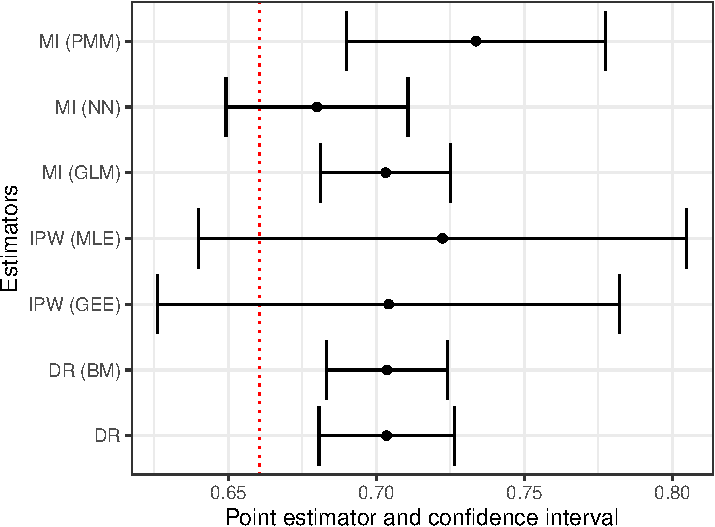
\includegraphics{nonprobsvy-paper_files/figure-latex/comparison-of-est-1} 

}

\caption[Comparison of estimates of the share of job vacancies offered on a single-shift]{Comparison of estimates of the share of job vacancies offered on a single-shift}\label{fig:comparison-of-est}
\end{figure}
\end{CodeChunk}

\subsection{Advanced usage}\label{advanced-usage}

\subsubsection{Bootstrap Approach for Variance
Estimation}\label{bootstrap-approach-for-variance-estimation}

In the package we allow user to estimate variance of the mean using
analytical (default) or bootstrap approach as described in Section
\ref{sec-prediction}. In case of analytical variance estimators we use
the estimators proposed in the papers described in the Section
\ref{sec-methods}. Users may disable standard error calculation using
\code{nonprob(se=FALSE)}. The bootstrap approach implemented in the
package refers to two samples:

\begin{itemize}
\item non-probability -- we currently support only simple random sampling with replacement,
\item probability -- we support all the approaches implemented in the \code{as.svrepdesign} and we refer the reader to the help file of this function. 
\end{itemize}

To specify the bootstrap approach one should use \code{control_inf()}
function with \texttt{var\_method\ =\ "bootstrap"}. Controlling the
bootstrap method for probability sample is done by \texttt{rep\_type}
argument which passes the method to the \texttt{as.svrepdesign}
function. The number of iterations is set in the \texttt{num\_boot}
argument (default 100). If the samples are large or the estimation
method is complicated (e.g.~involves variable selection) one can set
\texttt{verbose=TRUE} to track the progress. By default results of
bootstrap are stored in the \texttt{boot\_sample} element of the
resulting list (to disable this \texttt{keep\_boot} should be set to
\texttt{FALSE}). The following code provides an example of using the IPW
approach with the bootstrap approach specified by the argument
\texttt{control\_inference} of the \texttt{nonprob} function.

\begin{CodeChunk}
\begin{CodeInput}
R> ipw_est1_boot <- nonprob(
+   selection = ~ region + private + nace + size,
+   target = ~ single_shift,
+   svydesign = jvs_svy,
+   data = admin,
+   method_selection = "logit",
+   control_inference = control_inf(var_method = "bootstrap", num_boot = 50),
+   verbose = F
+ )
\end{CodeInput}
\end{CodeChunk}

Next, we compare the estimated standard error with the analytical one
below.

\begin{CodeChunk}
\begin{CodeInput}
R> rbind("IPW analytic variance"=ipw_est1$output,
+       "IPW bootstrap variance"=ipw_est1_boot$output)
\end{CodeInput}
\begin{CodeOutput}
                            mean          SE
IPW analytic variance  0.7083228 0.009436907
IPW bootstrap variance 0.7083228 0.010065839
\end{CodeOutput}
\end{CodeChunk}

To assess the samples one can access the \texttt{boot\_sample} element
of the output list of the \texttt{nonprob} function. Note that this is
returned as \texttt{matrix} because we allow multiple \texttt{target}
variables.

\begin{CodeChunk}
\begin{CodeInput}
R> head(ipw_est1_boot$boot_sample, n=3)
\end{CodeInput}
\begin{CodeOutput}
     single_shift
[1,]    0.7062196
[2,]    0.7116044
[3,]    0.7119409
\end{CodeOutput}
\end{CodeChunk}

\subsubsection{Variable Selection
Algorithms}\label{variable-selection-algorithms}

In this section we briefly present how to use variable selection
algorithms. In order to specify that a variable selection algorithm
should be used one should specify the
\texttt{control\_inference\ =\ control\_inf(vars\_selection\ =\ TRUE)}
argument. Then, the user should either leave the default or specify the
parameters for the outcome via the \code{control_out} function or
selection outcome (\code{control_sel}). Both function have the same
parameters:

\begin{itemize}
\item \code{penalty} -- The penalization function used during variables selection (possible values: \code{c("SCAD", "lasso", "MCP")})
\item \code{nlambda} -- The number of $\lambda$ values. Default is 50.
\item \code{lambda_min} -- The smallest value for $\lambda$, as a fraction of \code{lambda.max}. Default is .001.
\item \code{lambda} -- A user specified vector of lambdas (only for the \code{control_sel} function).
\item \code{nfolds} -- The number of folds for cross validation. Default is 10.
\item \code{a_SCAD, a_MCP} -- The tuning parameter of the SCAD and MCP penalty for selection model. Default is 3.7 and 3 respectively.
\end{itemize}

For the MI approach we leverage the \pkg{ncvreg} package \citep{ncvreg}
as it is solely package that uses the SCAD method in \proglang{R}. For
the IPW and DR approaches we have developed our own codes in
\proglang{C++} via the \pkg{Rcpp} and \pkg{RcppArmadillo} packages. In
the code below we apply variable selection for the MI GLM estimator
using only 5 folds, 25 possible values of \(\lambda\) parameters and
apply the LASSO penalty.

\begin{CodeChunk}
\begin{CodeInput}
R> mi_est1_sel <- nonprob(
+   outcome = single_shift ~ region + private + nace + size,
+   svydesign = jvs_svy,
+   data = admin,
+   method_outcome = "glm",
+   family_outcome = "binomial" ,
+   control_outcome = control_out(nfolds = 5, nlambda = 25, penalty = "lasso"),
+   control_inference = control_inf(vars_selection = TRUE),
+   verbose = TRUE
+ )
\end{CodeInput}
\begin{CodeOutput}
Starting CV fold #1
Starting CV fold #2
Starting CV fold #3
Starting CV fold #4
Starting CV fold #5
\end{CodeOutput}
\end{CodeChunk}

In this case study the MI GLM estimator with variable selection yields
almost the same results as the approach without it. Point estimates and
standard errors differ at the fourth and third digit respectively.

\begin{CodeChunk}
\begin{CodeInput}
R> rbind("MI without var sel"=mi_est1$output,
+       "MI with var sel"=mi_est1_sel$output)
\end{CodeInput}
\begin{CodeOutput}
                        mean         SE
MI without var sel 0.7032081 0.01120231
MI with var sel    0.7031075 0.01120569
\end{CodeOutput}
\end{CodeChunk}

\section[Classes and S3Methods]{Classes and \code{S3Methods}}\label{sec-s3methods}

In the package we have created the main class \code{nonprobsvy} and a
supplementary class \code{summary_nonprobsvy}. All \code{S3methods}
implemented can be obtained by using \code{methods(class="nonprobsvy")}.
For instance, the \code{check_balance} function already mentioned in the
case study allows to assess the balance by checking how the PS weights
reproduce known or estimated population totals, or the \code{nobs}
function returns the sample size of the probability and non-probability
samples:

\begin{CodeChunk}
\begin{CodeInput}
R> nobs(dr_est1)
\end{CodeInput}
\begin{CodeOutput}
   prob nonprob 
   6523    9344 
\end{CodeOutput}
\end{CodeChunk}

Table \ref{tab-s3methods} presents methods implemented for the
\code{nonprobsy} class. On purpose we did not implement many methods as
the goal of the package is to provide point and interval estimates. If a
user is interested in assessing the quality of the models or covariate
balance should use existing \proglang{R} packages.

\begin{table}[ht!]
\centering
\small
\begin{tabular}{p{4cm}p{11cm}}
\hline 
Function & Description \\
\hline
\code{check_balance} & aaa; \\
\code{confint} & aaa\\
\code{nobs} & \\
\code{pop_size} & \\
\code{summary} & \\
\code{logLik, AIC, BIC, deviance} & \\
\code{residuals, hatvalues, cooks.distance, print, vcov}  & it works exactly like \code{glm} counterparts.\\
\hline 
\end{tabular}
\caption{\code{S3Methods} implemented in the \pkg{nonprobsvy}}
\label{tab-s3methods}
\end{table}

\section{Summary and future work}\label{summary-and-future-work}

The \pkg{nonprobsvy} package provides a comprehensive R toolkit for
addressing inference challenges with non-probability samples by
integrating them with probability samples or known population
totals/means. As non-probability data sources like administrative data,
voluntary online panels, and social media data become increasingly
available, statisticians need robust methods to produce reliable
population estimates. The package implements \textit{state-of-the-art}
approaches including mass imputation, inverse probability weighting
(IPW), and doubly robust (DR) methods, each designed to correct
selection bias by leveraging auxiliary data. By providing a unified
framework and integration with the \pkg{survey} package,
\pkg{nonprobsvy} makes complex statistical methods for non-probability
samples more accessible, enabling researchers to produce robust
estimates even when working with non-representative data.

There are several avenues for future development of the \pkg{nonprobsvy}
package. A key priority is implementing model-based calibration and
additional methods for estimating propensity scores and weights. The
package currently assumes no overlap between probability and
non-probability samples, so accounting for potential overlap (e.g., in
big data sources and registers) is another important extension.
Additional planned developments include handling non-ignorable sample
selection through sample selection models, maintaining consistency with
calibration weights, and supporting multiple non-probability samples for
data integration from various sources.

Further methodological extensions under consideration include empirical
likelihood approaches for doubly/multiply robust estimation, integration
of machine learning methods like debiased/double machine learning from
causal inference, handling measurement error in big data variables, and
expanding the bootstrap approach beyond simple random sampling with
replacement. The package will also be extended to work with the
\texttt{svyrep.design} class from the \pkg{survey} package and the
\pkg{svrep} package. These developments will enhance \pkg{nonprobsvy}'s
capabilities for handling complex survey data structures and modern
estimation challenges.

\section{Acknowledgements}\label{sec-acknowledgements}

The authors' work has been financed by the National Science Centre in
Poland, OPUS 20, grant no. 2020/39/B/HS4/00941.

Łukasz Chrostowski is the main developer and maintainer of the package.
Parts of this paper are based on Łukasz's Master's thesis (available at
\url{https://github.com/ncn-foreigners/graduation-theses}). Piotr
Chlebicki contributed to the package and implemented MI-PMM estimators.
Maciej Beręsewicz was responsible for the initial idea and the design of
the package, testing, reviewing and small contributions code and
prepared the manuscript.

We would like to thank \ldots{}

\clearpage

\appendix

\section{List of symbols}\label{list-of-symbols}

\begin{table}[ht!]
\centering
\begin{tabular}{ll}
\hline
\textbf{Symbol} & \textbf{Description} \\
\hline
$U$ & Target population of size $N$ \\
$S_A$ & Non-probability sample \\
$S_B$ & Probability sample \\
$N$ & Population size \\
$n_A$ & Size of non-probability sample \\
$n_B$ & Size of probability sample \\
$\hat{N}^A$ & Estimated size based on non-probability sample \\
$\hat{N}^B$ & Estimated size based on probability sample \\
$\boldsymbol{x}_i$ & Vector of auxiliary variables for unit $i$ \\
$y_i$ & Value of the study/target variable for unit $i$ \\
$y_i^*$ & Imputed value for unit $i$ in $S_B$\\
$\pi_i^A$ & Propensity score for unit $i$ in non-probability sample \\
$\pi_i^B$ & Inclusion probability for unit $i$ in probability sample \\
$d_i^A$ & Inverse probability weight ($1/\pi_i^A$) for non-probability sample \\
$d_i^B$ & Design weight ($1/\pi_i^B$) for probability sample \\
$R_i^A$ & Indicator of inclusion into non-probability sample \\
$R_i^B$ & Indicator of inclusion into probability sample \\
$\mu$ & Population mean of target variable $y$ \\
$\mu_{\boldsymbol{x}}$ & Population means of auxiliary variables $\boldsymbol{x}$ \\
$m(\boldsymbol{x}_i, \boldsymbol{\beta})$ & Semiparametric model for outcome variable \\
$\dot{m}(\boldsymbol{x}_i, \boldsymbol{\beta})$ & First derivative of the $m(\boldsymbol{x}_i, \boldsymbol{\beta})$ with respect to $\boldsymbol{\beta}$ \\
$\pi(\boldsymbol{x}_i, \boldsymbol{\gamma})$ & Propensity score model for $R_i^A$ \\
$\boldsymbol{\beta}$ & Parameter vector for outcome model \\
$\boldsymbol{\gamma}$ & Parameter vector for propensity score model \\
$\lambda_{\boldsymbol{\beta}}, \lambda_{\boldsymbol{\gamma}}$ & Tuning parameters for penalisation methods \\
$\hat{\mu}_{\boldsymbol{x}}$ & Estimator for the population means of auxiliary variables $\boldsymbol{x}$ \\
$\bar{\boldsymbol{x}}_{A}$ & A vector of the sample means of the auxiliary variables $\boldsymbol{x}$ from $S_A$ \\ 
$\hat{\mu}_{PR}$ & Prediction estimators \\
$\hat{\mu}_{MI}$ & Mass imputation estimator \\
$\hat{\mu}_{IPW}$ & Inverse probability weighting estimator \\
$\hat{\mu}_{DR}$ & Doubly robust estimator \\
$\hat{V}_{boot}$ & Variance estimator based on the bootstrap \\
\hline
\end{tabular}
\caption{List of symbols and their descriptions}
\label{tab-list-of-symbols}
\end{table}

\clearpage

\section{Algorithms for the MI-NN and MI-PMM
estimators}\label{sec-details}

\begin{algorithm}[ht!]
\caption{Mass imputation using the k-nearest-neighbour algorithm}
\label{algo-2}
\begin{algorithmic}[1]
\State If $k=1$, then for each $i \in S_B$ match $\hat{\nu}(i)$ such that
$\displaystyle \hat{\nu}(i)=
\operatornamewithlimits{arg\,min}_{j\in S_{A}}d\left(\boldsymbol{x}_i,\boldsymbol{x}_j\right)$.
\State If $k>1$, then
$$\hat{\nu}(i, z) = \operatornamewithlimits{arg\,min}_{\displaystyle j\in S_{A}\setminus\bigcup_{t=1}^{z-1}
\{\hat{\nu}(i, t)\}} d\left(\boldsymbol{x}_i, \boldsymbol{x}_j\right)$$
i.e. $\hat{\nu}(i, z)$ is $z$-th nearest neighbour from the sample.\;
\State For each $i \in S_B$, calculate the imputed value as
$$
\hat{y}_i = \frac{1}{k}\sum_{t=1}^{k}y_{\hat{\nu}(i, t)}.
$$
\end{algorithmic}
\end{algorithm}

\begin{algorithm}[ht!]
\caption{$\hat{y}-\hat{y}$ Imputation:}
\label{algo-3}
\begin{algorithmic}[1]
\State Estimate regression model $\mathbb{E}[Y|\boldsymbol{X}=\boldsymbol{x}]=m(\boldsymbol{x}, \boldsymbol{\beta})$.\;
\State Impute $$\hat{y}_{i}=m\left(\boldsymbol{x}_{i},\hat{\boldsymbol{\beta}}\right), 
\hat{y}_{j}=m\left(\boldsymbol{x}_{j},\hat{\boldsymbol{\beta}}\right)$$
for $i\in S_{B}, j\in S_{A}$ and assign each 
$i\in S_{B}$ to $\hat{\nu}(i)$, where
$$\displaystyle \hat{\nu}(i)=
\operatornamewithlimits{arg\,min}_{j\in S_{A}}\lVert \hat{y}_{i}-\hat{y}_{j}\rVert$$ or
$$\displaystyle \hat{\nu}(i)=
\operatornamewithlimits{arg\,min}_{j\in S_{A}}d\left(\hat{y}_{i},\hat{y}_{j}\right)$$ if $d$ is not induced by the norm.\;

\State If $k>1$, then:
$$\hat{\nu}(i, z) = \operatornamewithlimits{arg\,min}_{\displaystyle j\in S_{A}\setminus\bigcup_{t=1}^{z-1}
\{\hat{\nu}(i, t)\}} d\left(\hat{y}_{i},\hat{y}_{j}\right)$$
e.g., $\hat{\nu}(i, z)$ is $z$-th nearest neighbor from a sample.\;
\State For $i \in S_B$, calculate imputation value as 
$$
\hat{y}_i = \frac{1}{k}\sum_{t=1}^{k}y_{\hat{\nu}(i, t)}.
$$
\end{algorithmic}
\end{algorithm}

\begin{algorithm}[ht!]
\caption{$\hat{y}-y$ Imputation:}
\label{algo-4}
\begin{algorithmic}[1]
\State Estimate regression $\mathbb{E}[Y|\boldsymbol{X}=\boldsymbol{x}]=m(\boldsymbol{x}, \boldsymbol{\beta})$.\;
\State Impute $\hat{y}_{i}=m\left(\boldsymbol{x}_{i},\hat{\boldsymbol{\beta}}\right)$ 
for $i \in S_{B}$ and assign each 
$i \in S_{B}$ do $\hat{\nu}(i)$, where
$\displaystyle \hat{\nu}(i)=
\operatornamewithlimits{arg\,min}_{j \in S_{A}}\lVert \hat{y}_{i}-y_{j}\rVert$ or
$\displaystyle \hat{\nu}(i)=
\operatornamewithlimits{arg\,min}_{j \in S_{A}}d\left(\hat{y}_{i},y_{j}\right)$ 
if $d$ not induced by the norm.\;
\State If $k>1$, then:
$$\hat{\nu}(i, z) = \operatornamewithlimits{arg\,min}_{\displaystyle j \in S_{A} \setminus \bigcup_{t=1}^{z-1}
\{\hat{\nu}(i, t)\}}
d\left(\hat{y}_{i},y_{j}\right).$$
\State For each $i \in S_B$ calculate imputation value as
$$
\hat{y}_i = \frac{1}{k}\sum_{t=1}^{k}y_{\hat{\nu}(i, t)}.
$$
\end{algorithmic}
\end{algorithm}

\newpage

\bibliography{references.bib}



\end{document}
